% PrivacyGNN — Project learning guide (general → specific)
% Build: pdflatex PROJECT_LEARNING_GUIDE.tex (run twice for stable references)
\documentclass[11pt,a4paper]{article}
\usepackage[margin=1in]{geometry}
\usepackage[T1]{fontenc}
\usepackage{lmodern}
\usepackage{microtype}
\usepackage{graphicx}
\usepackage{booktabs}
\usepackage{array}
\usepackage{amsmath}
\usepackage{xcolor}
\usepackage{hyperref}
\usepackage{tikz}
\usetikzlibrary{arrows.meta,positioning,shapes.multipart,calc}

\hypersetup{colorlinks=true,linkcolor=blue!60!black,urlcolor=blue!60!black,citecolor=blue!60!black}
% Tighter lists without enumitem (works on minimal TeX installs)
\makeatletter
\def\@listi{\leftmargin\leftmargini \topsep 2pt \parsep 2pt \itemsep 2pt}
\makeatother

\title{\textbf{PrivacyGNN}\\[0.4em]
\large A learner's guide to the whole project\\[0.2em]
\normalsize From research goals to code and outputs}
\author{Krish Sharma (with PI Dr.\ Shaikh Arifuzzaman)}
\date{\today}

\begin{document}
\maketitle
\begin{abstract}
\noindent
This guide explains the \textbf{PrivacyGNN} codebase in plain language: what problem it studies, how the pieces connect, and where to look in the repository. It moves from the big picture (privacy and graph learning) down to files, configuration, metrics, and known limitations of this checkout. Read it once top-to-bottom, then use the file index as a map when you dive into code.
\end{abstract}
\tableofcontents
\newpage

%==============================================================================
\section{The big picture: what this project is}
%==============================================================================

\textbf{PrivacyGNN} is a research codebase that asks: \emph{Do graph neural networks (GNNs) leak information about which data points were used for training?} That question is formalized with \textbf{membership inference attacks} (MIAs): algorithms that try to guess whether a given example was in the training set, using only the trained model's predictions (or related signals).

The project compares:
\begin{itemize}
  \item \textbf{Graph models} (GCN, GraphSAGE) that use both node features and edges, versus
  \item \textbf{Non-graph baselines} (logistic regression, MLP) that use features only.
\end{itemize}
It also tests whether simple \textbf{defenses} (DropEdge, label smoothing, early stopping, confidence masking, edge sparsification, and an optional DP-SGD-style path) reduce attack success without destroying task accuracy.

\begin{center}
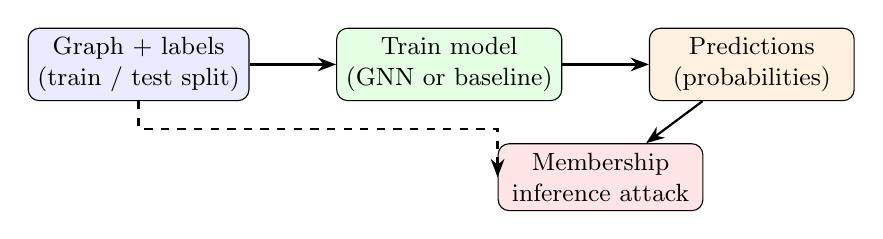
\begin{tikzpicture}[
  font=\small,
  box/.style={draw,rounded corners,align=center,minimum width=2.6cm,minimum height=0.85cm},
  arr/.style={-{Stealth},thick}
]
\node[box,fill=blue!8] (data) {Graph + labels\\(train / test split)};
\node[box,fill=green!10,right=1.1cm of data] (model) {Train model\\(GNN or baseline)};
\node[box,fill=orange!12,right=1.1cm of model] (pred) {Predictions\\(probabilities)};
\node[box,fill=red!10,below=1cm of $(model)!0.5!(pred)$] (atk) {Membership\\inference attack};
\draw[arr] (data) -- (model);
\draw[arr] (model) -- (pred);
\draw[arr] (pred) -- (atk);
\draw[arr,dashed] (data.south) -- ++(0,-0.35) -| (atk.west);
\end{tikzpicture}
\end{center}
\textit{Figure: Training produces a model; attacks use outputs (and implicitly know train vs.\ test membership for evaluation). The dashed line reminds you that the \emph{attacker} in the real world does not see ground-truth membership---we only use it to score the attack.}

%==============================================================================
\section{Why graphs make privacy interesting}
%==============================================================================

On images or tabular rows, each training example is often independent. On a \textbf{graph}, nodes are linked: a node's prediction depends on its neighbors. So ``membership'' is entangled with structure---a node's training signal propagates through edges. This project measures leakage in that setting and relates it to measurable graph statistics:
\begin{itemize}
  \item \textbf{Homophily:} fraction of edges connecting same-label nodes (high = neighbors tend to agree).
  \item \textbf{Density:} how many edges exist relative to all possible edges.
\end{itemize}
Synthetic datasets in \texttt{data.py} vary homophily (\texttt{high} / \texttt{low}) and density (\texttt{sparse} / \texttt{medium} / \texttt{dense}) \emph{orthogonally}, so you can study structure effects in a controlled way. Citation networks (Cora, Citeseer) provide realistic benchmarks.

%==============================================================================
\section{Research questions (what the experiments answer)}
%==============================================================================

\begin{enumerate}
  \item \textbf{RQ1:} Are GNNs more vulnerable to MIAs than non-graph baselines (MLP / logistic regression)?
  \item \textbf{RQ2:} How do homophily and density correlate with leakage?
  \item \textbf{RQ3:} Do lightweight defenses reduce leakage with acceptable utility loss?
  \item \textbf{RQ4:} What does the utility--privacy tradeoff look like?
\end{enumerate}
The pipeline produces accuracy, F1, AUROC (task performance), several attack AUC/accuracy scores, and calibration error (ECE) so you can relate \emph{utility} and \emph{privacy} numerically.

%==============================================================================
\section{Repository map (what lives where)}
%==============================================================================

The active code lives under \texttt{privacy-gnn/}. Think of it in layers:

\begin{center}
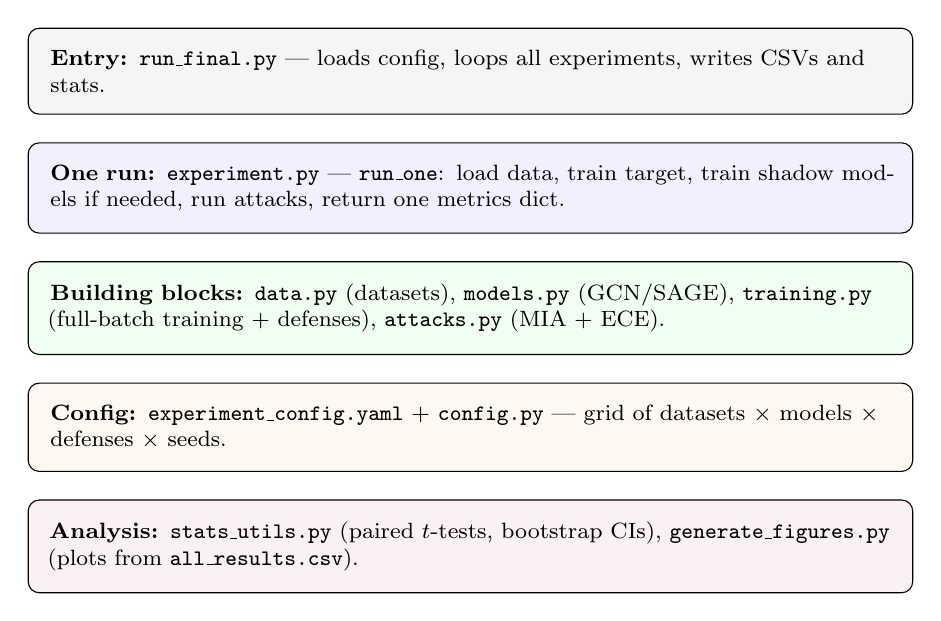
\begin{tikzpicture}[
  font=\footnotesize,
  layer/.style={draw,rounded corners,align=left,text width=0.88\textwidth,inner sep=8pt}
]
\node[layer,fill=gray!8] (L1) {\textbf{Entry:} \texttt{run\_final.py} --- loads config, loops all experiments, writes CSVs and stats.};
\node[layer,fill=blue!6,below=0.35cm of L1] (L2) {\textbf{One run:} \texttt{experiment.py} --- \texttt{run\_one}: load data, train target, train shadow models if needed, run attacks, return one metrics dict.};
\node[layer,fill=green!6,below=0.35cm of L2] (L3) {\textbf{Building blocks:} \texttt{data.py} (datasets), \texttt{models.py} (GCN/SAGE), \texttt{training.py} (full-batch training + defenses), \texttt{attacks.py} (MIA + ECE).};
\node[layer,fill=orange!6,below=0.35cm of L3] (L4) {\textbf{Config:} \texttt{experiment\_config.yaml} + \texttt{config.py} --- grid of datasets $\times$ models $\times$ defenses $\times$ seeds.};
\node[layer,fill=purple!6,below=0.35cm of L4] (L5) {\textbf{Analysis:} \texttt{stats\_utils.py} (paired $t$-tests, bootstrap CIs), \texttt{generate\_figures.py} (plots from \texttt{all\_results.csv}).};
\end{tikzpicture}
\end{center}

\noindent\textbf{Paper assets:} \texttt{paper/ieee\_privacy\_gnn.tex}, \texttt{paper/build\_manuscript.py}, and related notes (\texttt{JOURNAL\_REPORT.md}, \texttt{literature\_review.md}).

%==============================================================================
\section{Configuration-driven experiments}
%==============================================================================

You rarely need to edit Python to change the experimental grid. \texttt{config.py} reads \texttt{experiment\_config.yaml} (or the path in environment variable \texttt{PRIVACYGNN\_CONFIG}).

\textbf{Key YAML sections:}
\begin{itemize}
  \item \texttt{seeds} --- list of random seeds (each full combination runs once per seed).
  \item \texttt{datasets} --- e.g.\ \texttt{Cora}, \texttt{Citeseer}, \texttt{synthetic\_high\_sparse}, \ldots
  \item \texttt{models} --- \texttt{LogReg}, \texttt{MLP}, \texttt{GCN}, \texttt{GraphSAGE}.
  \item \texttt{defenses} --- list of \texttt{name} + \texttt{params}; \texttt{none} is the baseline.
  \item \texttt{attacks} --- which MIAs to run: \texttt{confidence}, \texttt{threshold}, \texttt{shadow}, \texttt{lira}.
  \item \texttt{training} --- epochs, learning rate, weight decay passed into \texttt{run\_one}.
  \item \texttt{bootstrap}, \texttt{lira}, \texttt{minibatch}, \texttt{dp\_sgd} --- advanced options (see below).
\end{itemize}

\textbf{Rules enforced in code} (\texttt{get\_experiment\_list} in \texttt{config.py}):
\begin{itemize}
  \item LogReg and MLP only run with defense \texttt{none} (graph-specific defenses apply to GNNs).
  \item Defense \texttt{dp\_sgd} only applies to \texttt{GCN} and \texttt{GraphSAGE}, and optionally only on datasets listed in \texttt{dp\_sgd\_datasets}.
\end{itemize}

For a smaller, paper-aligned grid, use \texttt{experiment\_config\_paper.yaml}:
\begin{verbatim}
PRIVACYGNN_CONFIG=experiment_config_paper.yaml python run_final.py
\end{verbatim}

%==============================================================================
\section{Data: real graphs and synthetic controls}
%==============================================================================

\textbf{Cora / Citeseer} (\texttt{load\_citation}): loaded via PyTorch Geometric Planetoid; a mirror URL is tried if the default download fails.

\textbf{Synthetic graphs} (\texttt{make\_synthetic}): fixed number of nodes and features; labels drawn from class centers; edges sampled to hit a target density, with a controllable fraction of same-label vs.\ different-label edges (homophily). Train/test is a 50/50 split (with optional \texttt{resplit} for new splits per seed).

\textbf{Large-graph path} (\texttt{ogb\_loader.py}, \texttt{graph\_minibatch.py}): in \emph{this repository snapshot}, \texttt{MINIBATCH\_DATASETS} is empty and minibatch/DP functions raise \texttt{NotImplementedError}. The YAML may mention \texttt{ogbn-arxiv} or Reddit as future extensions; the learning guide reflects the code as checked in.

%==============================================================================
\section{Models and training}
%==============================================================================

\textbf{GNNs} (\texttt{models.py}): two-layer GCN and GraphSAGE (64 hidden units), dropout between layers.

\textbf{Training} (\texttt{training.py}, full-batch): Adam, cross-entropy on masked training nodes. Optional:
\begin{itemize}
  \item \textbf{DropEdge:} randomly drop edges each epoch during training.
  \item \textbf{Label smoothing:} replace one-hot targets with softened distributions.
  \item \textbf{Early stopping:} track training loss improvement; restore best weights.
  \item \textbf{Edge sparsification:} remove a fraction of edges once before training.
\end{itemize}

\textbf{Baselines:} logistic regression and sklearn MLP fit on node features only (no graph), in \texttt{experiment.py}.

\textbf{Confidence masking} is applied to \emph{predicted probabilities} after training: keep only top-$k$ class masses and renormalize, to obscure fine-grained confidence.

%==============================================================================
\section{Membership inference attacks (how leakage is measured)}
%==============================================================================

All attacks here are \textbf{evaluated} using the known train/test split: training nodes are labeled ``member'' and test nodes ``non-member.'' The attacker sees model outputs and tries to classify membership. Attack AUC $= 0.5$ means no better than random; higher AUC suggests more leakage.

\textbf{Feature vector} (four dimensions, \texttt{extract\_features} in \texttt{attacks.py}) per node:
\begin{enumerate}
  \item Maximum predicted probability.
  \item Predicted probability of the \emph{true} label.
  \item Entropy of the predictive distribution.
  \item A confidence margin term derived from max probability.
\end{enumerate}

\textbf{Confidence attack:} train a logistic regression to distinguish members vs.\ non-members using these features; report AUC and accuracy on a held-out half of the combined set.

\textbf{Threshold attack:} uses true-label confidence only, with a median threshold (also returns AUC/acc).

\textbf{Shadow-model attack:} train the same type of model on a \emph{shadow} dataset (same family as the target, different random split/seed), build features from shadow member/non-member predictions, train an attack model, then evaluate on the \emph{target} model's members and non-members.

\textbf{LiRA slot:} config may include \texttt{lira}. In this checkout, \texttt{lira\_attack.py} returns chance-level $0.5$ / $0.5$ as a placeholder when a full LiRA implementation is not present.

\textbf{ECE:} expected calibration error on test predictions (\texttt{calibration\_error})---not an attack, but relates to how ``trustable'' confidences are.

%==============================================================================
\section{One experiment end-to-end (\texttt{run\_one})}
%==============================================================================

\begin{enumerate}
  \item Load dataset and compute homophily and density statistics.
  \item Set random seeds (NumPy, PyTorch).
  \item Build defense-specific training kwargs (DropEdge rate, etc.).
  \item Train the \textbf{target} model; obtain full-graph probabilities (or baseline \texttt{predict\_proba}).
  \item Apply confidence masking to probabilities if configured.
  \item Compute task metrics on the test mask: accuracy, macro F1, multiclass AUROC (with fallback).
  \item If enabled, run confidence/threshold attacks comparing train vs.\ test outputs.
  \item If shadow/LiRA need shadows, train one or more shadow models with independent seeds/splits, collect their probabilities, then run shadow attack and/or LiRA placeholder.
  \item Compute ECE on test predictions.
  \item Return a flat dictionary of metrics (one row for CSV).
\end{enumerate}

%==============================================================================
\section{Running the project and outputs}
%==============================================================================

\textbf{Setup:}
\begin{verbatim}
cd privacy-gnn
pip install -r requirements.txt
python run_final.py
\end{verbatim}

\textbf{Main outputs} (under \texttt{results/} unless overridden):
\begin{itemize}
  \item \texttt{all\_results.csv} --- one row per (dataset, model, defense, seed).
  \item \texttt{summary.csv} --- aggregated mean/std by (dataset, model, defense).
  \item \texttt{significance.csv} --- exploratory paired $t$-tests: each defense vs.\ \texttt{none} on attack AUC (\texttt{conf\_attack\_auc}), matched by seed.
  \item \texttt{significance\_lira.csv} --- same for LiRA AUC if column exists.
  \item \texttt{summary\_bootstrap.csv} --- bootstrap confidence intervals over seeds (not $p$-values).
  \item \texttt{all\_results.partial.csv} --- periodic checkpoint during long runs.
\end{itemize}

\textbf{Figures:} \texttt{python generate\_figures.py} reads \texttt{all\_results.csv} and writes PNGs to \texttt{figures/}.

\textbf{Manuscript PDF:} \texttt{python paper/build\_manuscript.py} (see \texttt{paper/}).

%==============================================================================
\section{How to read the results columns}
%==============================================================================

\begin{table}[ht]
\centering
\footnotesize
\setlength{\tabcolsep}{4pt}
\begin{tabular}{@{}>{\raggedright\arraybackslash}p{0.34\textwidth}p{0.58\textwidth}@{}}
\toprule
\textbf{Column} & \textbf{Meaning} \\
\midrule
\texttt{homophily}, \texttt{density} & Graph statistics for that run. \\
\texttt{test\_accuracy}, \texttt{test\_f1}, \texttt{test\_auroc} & Task utility on test nodes. \\
\texttt{conf\_attack\_auc}, \texttt{conf\_attack\_acc} & Classifier-based MIA. \\
\texttt{threshold\_attack\_auc}, \texttt{threshold\_attack\_acc} & Threshold on true-label confidence. \\
\texttt{shadow\_attack\_auc}, \texttt{shadow\_attack\_acc} & Shadow-model MIA. \\
\texttt{lira\_attack\_*} & LiRA metrics (placeholder $\approx 0.5$ in this checkout). \\
\texttt{ece\_test} & Calibration error (lower is better calibrated). \\
\texttt{dp\_epsilon} & Privacy budget if \texttt{dp\_sgd} ran (NaN otherwise). \\
\bottomrule
\end{tabular}
\end{table}

%==============================================================================
\section{Mental model: experiment grid size}
%==============================================================================

The total number of runs is approximately
\[
N_{\text{runs}} \approx
(\#\text{datasets}) \times (\#\text{models}) \times (\#\text{valid defenses}) \times (\#\text{seeds}),
\]
where ``valid defenses'' excludes combinations the code skips (for example, graph-only defenses on LogReg/MLP). The default YAML uses many seeds and defenses, so the full grid can be hundreds of runs---plan runtime accordingly or trim the YAML for development.

%==============================================================================
\section{Known limitations in this checkout (honest map)}
%==============================================================================

\begin{itemize}
  \item \textbf{Large-graph / OGB / Reddit:} not wired in this snapshot; stubs raise errors if selected.
  \item \textbf{LiRA:} placeholder returns chance-level scores; interpret \texttt{lira\_*} accordingly.
  \item \textbf{Statistical tests:} paired $t$-tests are \emph{exploratory}; bootstrap CIs quantify uncertainty over seeds but are not hypothesis tests.
  \item \textbf{DP-SGD:} would require the minibatch DP path in \texttt{graph\_minibatch.py} in a full implementation.
\end{itemize}

%==============================================================================
\section{Suggested learning path for you}
%==============================================================================

\begin{enumerate}
  \item Read this PDF once (general $\rightarrow$ specific).
  \item Open \texttt{experiment\_config.yaml} and trace one triple (dataset, model, defense) you care about.
  \item Read \texttt{run\_final.py} (loop) then \texttt{experiment.run\_one} (single run).
  \item Read \texttt{attacks.py} to internalize the four-dimensional feature map.
  \item Skim \texttt{data.make\_synthetic} to see how homophily and density are enforced.
  \item Run a \emph{tiny} grid: one synthetic dataset, two models, two defenses, two seeds---inspect \texttt{all\_results.csv}.
  \item Run \texttt{generate\_figures.py} and match each figure to filters in the plotting code.
\end{enumerate}

\vspace{1em}
\noindent\textit{End of guide.} For publication narrative and citations, align with \texttt{paper/ieee\_privacy\_gnn.tex} and your advisor's framing of contributions.

\end{document}
